\documentclass{article}
\usepackage[utf8]{inputenc}
\usepackage{mathptmx}
\usepackage{microtype}

\usepackage{graphicx}
\graphicspath{{images/}}
\usepackage{subcaption}
\usepackage{float}
\usepackage{amsmath}

\usepackage{listings}
\lstdefinestyle{withframe}{frame=single}
\lstset{style=withframe}

\title{CS5234 Project Report}

\author{
  Chan Wai Hap (Axxxxxx) \\
  \texttt{xxxxx@u.nus.edu}
  \and
  Lu Wei (A0040955E) \\
  \texttt{wei.lu@u.nus.edu}
}

\begin{document}

\maketitle

\tableofcontents

\pagebreak

\section{Overview}
The density of a graph is defined as the number of edges divided by the number of nodes.

\begin{equation}
  \rho(G) = \frac{m}{n}
\end{equation}

Where $m$ is the number of edges and $n$ is the number of nodes of graph $G$. This is a convention we are going to use consistently for the rest of this report.

A dense subgraph is induced by a set of nodes in the original graph with many edges connecting them. The problem of finding the densest subgraph for undirected graphs is first formalized by A. V. Goldberg in 1984 (REFERENCE). He proposed a polynomial time exact algorithm for both unweighted and weighted graphs. It has been an active area research since. This class of problems are interesting not just from a theoretical perspective, they also have a lot of practical applications, such as community detection in social networks, web link spam detection for search engines, and correlation mining for gene, item or time series datasets. Such graph datasets are usually large with millions and even billions of nodes, which makes poly-time algorithm impractical. This prompts research in the direction of both distributed and approximation algorithms.

In our project, we limit the scope of our investigation to unweighted and undirect graphs. First, we explored both exact and approximation algorithms from existing literature for the densest subgraph problem, and formulated a distributed exact algorithm. For experimentation, we implemented Goldberg's exact algorithm, which we used to produce baselines for various datasets we experimented with. We then replicated and improved a MapReduce implementation of an approximation algorithm by Bahman et al in Hadoop – a distributed big data processing framework built on top of the MapReduce computational model. Last but not least, we also adopted the same approximation algorithm to a distributed graph processing framework named Giraph. We will present challenges and key lessons learned and compare the Hadoop and Giraph implementations.

\section{Algorithms and Theory}
In this section, we will introduce Goldberg's exact algorithm and briefly cover several approximation algorithms. Lastly, we will present our distributed exact algorithms and two possible realizations.

\subsection{Exact Algorithm}
The key idea of Goldberg's exact algorithm is to convert the original undirected, unweighted graph into a flow network as illustrated below:

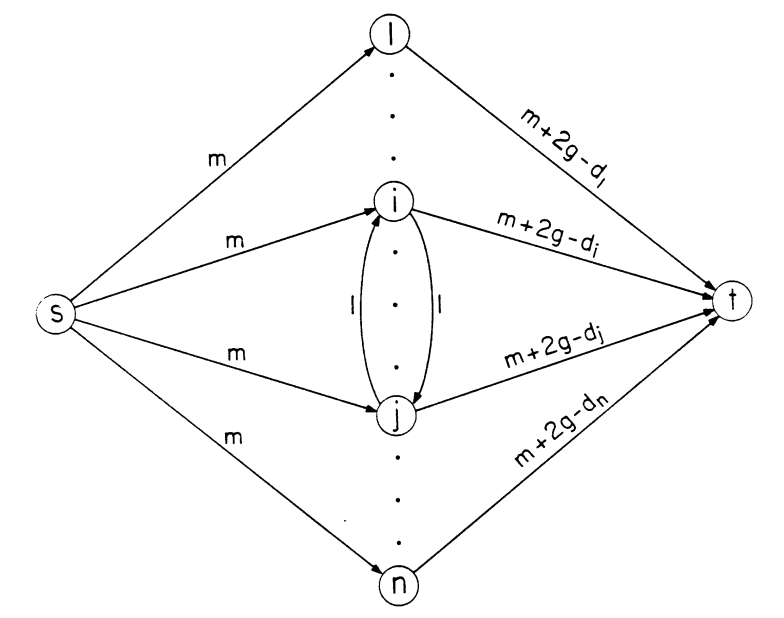
\includegraphics[width=\columnwidth]{goldberg_network.png}

Comparing to the original graph with nodes $V$ and edges $E$, the network has two nodes added: the source $s$ and the sink $t$: $V_N = V + \{s, t\}$, and $m + 2n$ edges added: $|E_N| = 2|E| + 2|N| = 2m + 2n$. Every original unweight and undirected edge is converted to two directed edges each with capacity 1. The capacity from $s$ to every node in the original graph is $m$; and the capacity from every node $i$ in the original graph to $t$ is assigned $m + 2g - d_i$, where $d_i$ is the degree of node $i$ in the original graph, and $g$ is a guessed value which the algorithm is going to iteratively ``sandwich'' by finding the min-cut until $g$ converges to the density of the densest subgraph.

The pseudocode for the algorithm is as below:

\begin{lstlisting}[mathescape=true]
  l=0, u=m, $V_1 = \emptyset$
  while $u - l > \frac{1}{n(n-1)}$ do
    $g = \frac{u+l}{2}$
    Construct network the updated g: $N = (V_N, E_N, g)$
    Find min-cut (S, T)
    if S = \{s\}
      u = g
    else
      l = g
      $V_1 = S - {s}$
  end
\end{lstlisting}

The intuition here is that the min-cut either goes throught all the out-edges of source node $s$, which looks like Case 1 below, or it doesn't (Case 2). In Case 1, the min-cut $c(S, T) = mn$; while for Case 2, the min-cut $c(S, T) = mn + 2n_1(g - \rho_1)$, where $n_1$ is the number of nodes in the subgraph induced by $V_1$ and $\rho_1$ is the density of the same subgraph. For detailed derivation please refer to the original paper (REFERENCE). Notice that the $mn$ term appears in both cases, so for Case 2 to be the min-cut, it has to be the case that $2n_1(g - \rho_1) < 0 \Rightarrow g < \rho_1 \leq \rho^*$ where $\rho^*$ is the densest subgraph density. It follows that when Case 1 is the min-cut, $g > \rho^*$.

\begin{figure}[H]
  \centering
  \begin{subfigure}{.48\textwidth}
    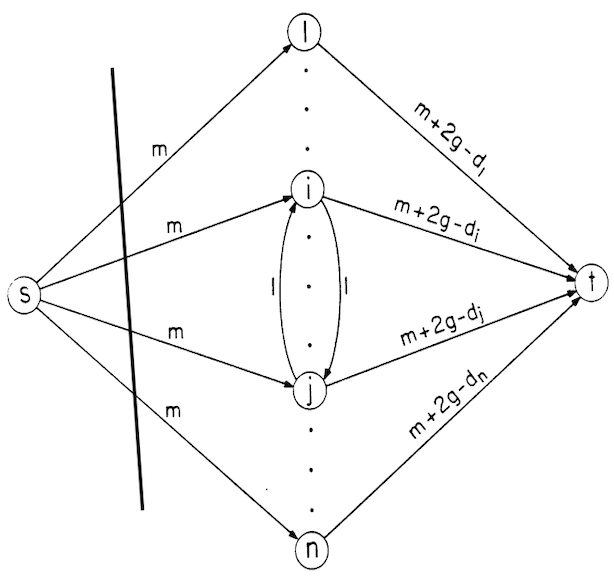
\includegraphics[width=\textwidth]{goldberg_network_cut1.png}
    \caption{Case 1}
  \end{subfigure}
  \begin{subfigure}{.48\textwidth}
    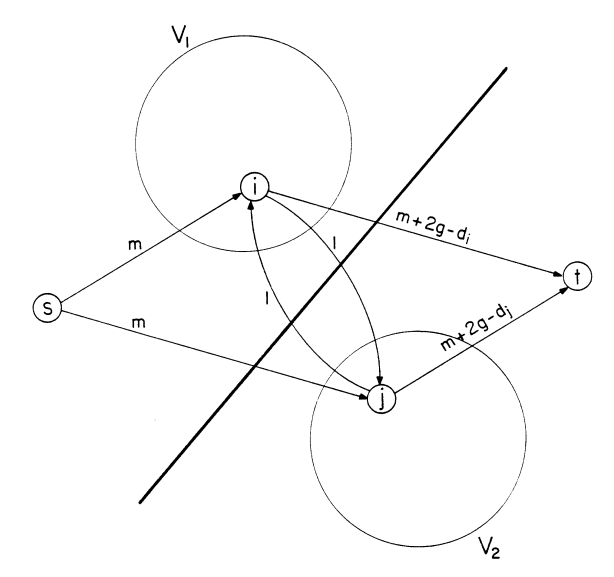
\includegraphics[width=\textwidth]{goldberg_network_cut2.png}
    \caption{Case 2}
  \end{subfigure}
\end{figure}

Since the value of $g$ is determined through binary search in the range of $[\frac{1}{n(n-1)}, m]$, it requires $log(n(n-1) \cdot m) = O(log(n^4)) = O(logn)$ iterations to terminate. Each iteration's running time is bounded by the time spent finding the min-cut in the contructed flow network.

There's extensive literature on finding s-t min-cut. The best known exact algorithm for general graphs is by Nagamochi and Ibaraki, which runs in time $O(mn + n^2logn)$ (REFERENCE). In comparison, the classic push-relabel algorithm by Goldberg and Tarjan (REFERENCE) runs in $O(n^3)$ time for a sequential implementation. Therefore for very dense subgraphs $m \approx n^2$, the best known min-cut algorithm's time complexity is also bounded by $O(n^3)$. Using $O(n^3)$ as the upper bound, the Goldberg densest subgraph algorithm described above has running time of $O(n^3logn)$.

We apprciate the cleverness of this algorithm in which one graph problem (densest subgraph) is translated to another graph problem (min-cut) through converting the original graph to a network flow with carefully assigned capacities. This is a common and effective technique we have come across while conducting literature review for this project.

\subsection{Approximation Algorithms}
We would like to focus on one approximation algorithm for finding densest subgraph in this section. It is proposed by Bahmani, Kumar, and Vassilvitskii (REFERENCE). The algorithm provides a $2 + 2\varepsilon$ approximation solution that completes in $O((m+n)logn$ time for a sequential implementation. We find this algorithm most impressive among its kind for the following reasons:

\begin{enumerate}
  \item Its distributed implementation completes in $O(logn)$ rounds,
  \item The algorithm itself is extremely simple, and
  \item It provides great close-to-truth approximation on real-world data.
\end{enumerate}

The key idea of this algorithm is to repeatedly remove small-degree nodes until the graph is empty. The intermediate subgraph with the highest density is the approximate solution to the densest subgraph problem. Below is the pseudocode:

\begin{lstlisting}[mathescape=true]
  $V_S, \tilde{V} = V$
  while $V_S \neq \emptyset$ do
    $V_R = \{i \in V_S | deg_S(i) \leq 2(1+\varepsilon)\rho_S\}$
    $V_S = V_S \ V_R$
    if $\tilde{\rho} < \rho_S$
      $\tilde{V} = V_S$
  end
\end{lstlisting}

Intuitively, this algorithm works because dense graph has large average degree, $\rho(G) = \frac{m}{n} = \frac{\sum_{i \in V}{deg_G(i)}}{2n} = \frac{1}{2} \textit{(average degree)}$. Therefore by removing small degree nodes, we expect the density of the subgraph induced by the remaining nodes to be large. The correctness and approximation bounds are established by setting the degree threshold carefully.

Let $V^*$ be the set of nodes in the true densest subgraph, $\rho^*$ be the true density. Removing any node i from $V^*$ will weakly reduce the density: $\rho^* \geq \rho(V^* \ \{i\}) = \frac{m^* - deg_{V^*}(i)}{n^* - 1}$. Since $n^* > 1$, we can multiply $n^* - 1$ on both sides of the inequality:

\begin{equation}
  \begin{split}
    \rho^* \cdot n^* - \rho^* & \geq m^* - deg_{V^*}(i) \\
    m^* - \rho^* & \geq m^* - deg_{V^*}(i) \\
    \rho^* & \leq deg_{V^*}(i)
  \end{split}
\end{equation}

Let i be a node in the true densest subgraph $ i \in V^*$, but we removed from $V_S$: $i \notin V_S$. This is bound to happen as $V_S$ is empty in the end. Since $V^* \subset V_S$ and i is removed because $deg_{V_S}(i) \leq 2(1+\varepsilon)\rho_S$. Combined with the inequality above, we have $\rho^* \leq deg_{V^*}(i) \leq deg_{V_S}(i) \leq 2(1+\varepsilon)\rho_S$, dividing $2(1+\varepsilon)$ on both sides:

\begin{equation}
  \rho_S \geq 2(1+\varepsilon) \rho^*
\end{equation}

This proves that the algorithm produces a $2(1+\varepsilon)$ approximation solution.

We can see that for every round of the algorithm, it reduces the graph size by a factor of at least $1+\varepsilon$. For node $i \in V_{St}$:

\begin{equation}
  \begin{split}
    \sum{deg_{V_{St}}(i)} & \geq n_{St} 2(1+\varepsilon)\rho_{S(t-1)} \\
    2 m_{S(t-1)} > \sum{deg_{V_{St}}(i)} & \geq n_{St} 2(1+\varepsilon) \frac{m_{S(t-1)}}{n_{S(t-1)}} \\
    \frac{n_{S(t-1)}}{n_{St}} & \geq (1+\varepsilon)
  \end{split}
\end{equation}

Therefore the algorithm terminates in $O(log_{(1+\varepsilon)}n)$ rounds. At each round, we check every node, which needs to count all its neighboring edges to get its degree, so the work per round is $O(m+n)$. Since degree is a node local property, the algorithm can therefore be distributed at every round.

\subsection{Distributed Exact Algorithms}

\section{Implementations and experiments}
\subsection{Hadoop Implementation \& Improvement}
\subsection{Giraph Adaptation}

\section{Conclusion}

\end{document}
